%%%%%%%%%%%%%%%%%%%%%%%%
%
% $Autor: Hemanth Jadiswami Prabhakaran $
% $Datum: 2025-06-30 11:19:07Z $
% $Pfad: GitHub/BA25-01-Time-Series/Manual/Chapters/en/05ApplicationFunctionsAndFeatures.tex $
% $Version: 1 $
%
% $Project: BA25-Time-Series $
%
%%%%%%%%%%%%%%%%%%%%%%%%



\chapter{Application Functions and Features}

\section{Comprehensive Feature Overview}

The Walmart Sales Forecasting System provides a complete ecosystem for time series forecasting, encompassing model development, training, evaluation, and production deployment. This chapter details every feature and function available across both applications.

\begin{figure}[H]
	\centering
	\begin{tikzpicture}[
	node distance=2.5cm,
	core/.style={ellipse, draw, fill=red!20, text width=3cm, text centered, minimum height=1.5cm},
	feature/.style={rectangle, draw, fill=blue!20, text width=2.5cm, text centered, rounded corners, minimum height=1cm},
	data/.style={rectangle, draw, fill=green!20, text width=2cm, text centered, rounded corners, minimum height=0.8cm},
	arrow/.style={thick,->,>=stealth}
	]
	
	% Title

	
	% Core system
	\node[core] (core) at (0,0) {\textbf{Walmart Sales\\Forecasting}};
	
	% Training Features (Left side)
	\node[feature] (training) at (-3.5,1.5) {Data Upload\\+ Training};
	\node[feature] (model_save) at (-3.5,-1.5) {Model Export};
	
	% Prediction Features (Right side)  
	\node[feature] (forecasting) at (3.5,1.5) {Load Model\\+ Forecast};
	\node[feature] (results) at (3.5,-1.5) {Visualization\\+ Export};
	
	% Data inputs (Top)
	\node[data] (input_data) at (0,3) {CSV Data Files};
	
	% Outputs (Bottom)
	\node[data] (output_data) at (0,-3) {Results + Charts};
	
	% Main connections
	\draw[arrow] (input_data) -- (training);
	\draw[arrow] (training) -- (core);
	\draw[arrow] (core) -- (model_save);
	\draw[arrow, dashed] (model_save) to[bend left=45] (forecasting);
	\draw[arrow] (forecasting) -- (core);
	\draw[arrow] (core) -- (results);
	\draw[arrow] (results) -- (output_data);
	
\end{tikzpicture}
	\caption{Complete Feature Ecosystem Overview}
	\label{fig:feature_ecosystem}
\end{figure}

\section{Training Application Functions}

\subsection{Data Management Features}

\subsubsection{Multi-File Data Upload}

The Training Application supports comprehensive data ingestion:

\textbf{Supported File Formats}
\begin{itemize}
	\item \textbf{CSV Files}: Primary format for all datasets
	\item \textbf{Encoding}: UTF-8 encoding support
	\item \textbf{Size Limits}: Up to 200MB per file (cloud), unlimited (local)
	\item \textbf{Validation}: Automatic schema validation upon upload
\end{itemize}

\textbf{Required Dataset Structure}
\begin{enumerate}
	\item \textbf{train.csv}: Historical sales data with Store, Date, Weekly\_Sales, IsHoliday
	\item \textbf{features.csv}: External factors with Store, Date, Temperature, Fuel\_Price, etc.
	\item \textbf{stores.csv}: Store metadata with Store, Type, Size information
\end{enumerate}

\begin{figure}[H]
	\centering
	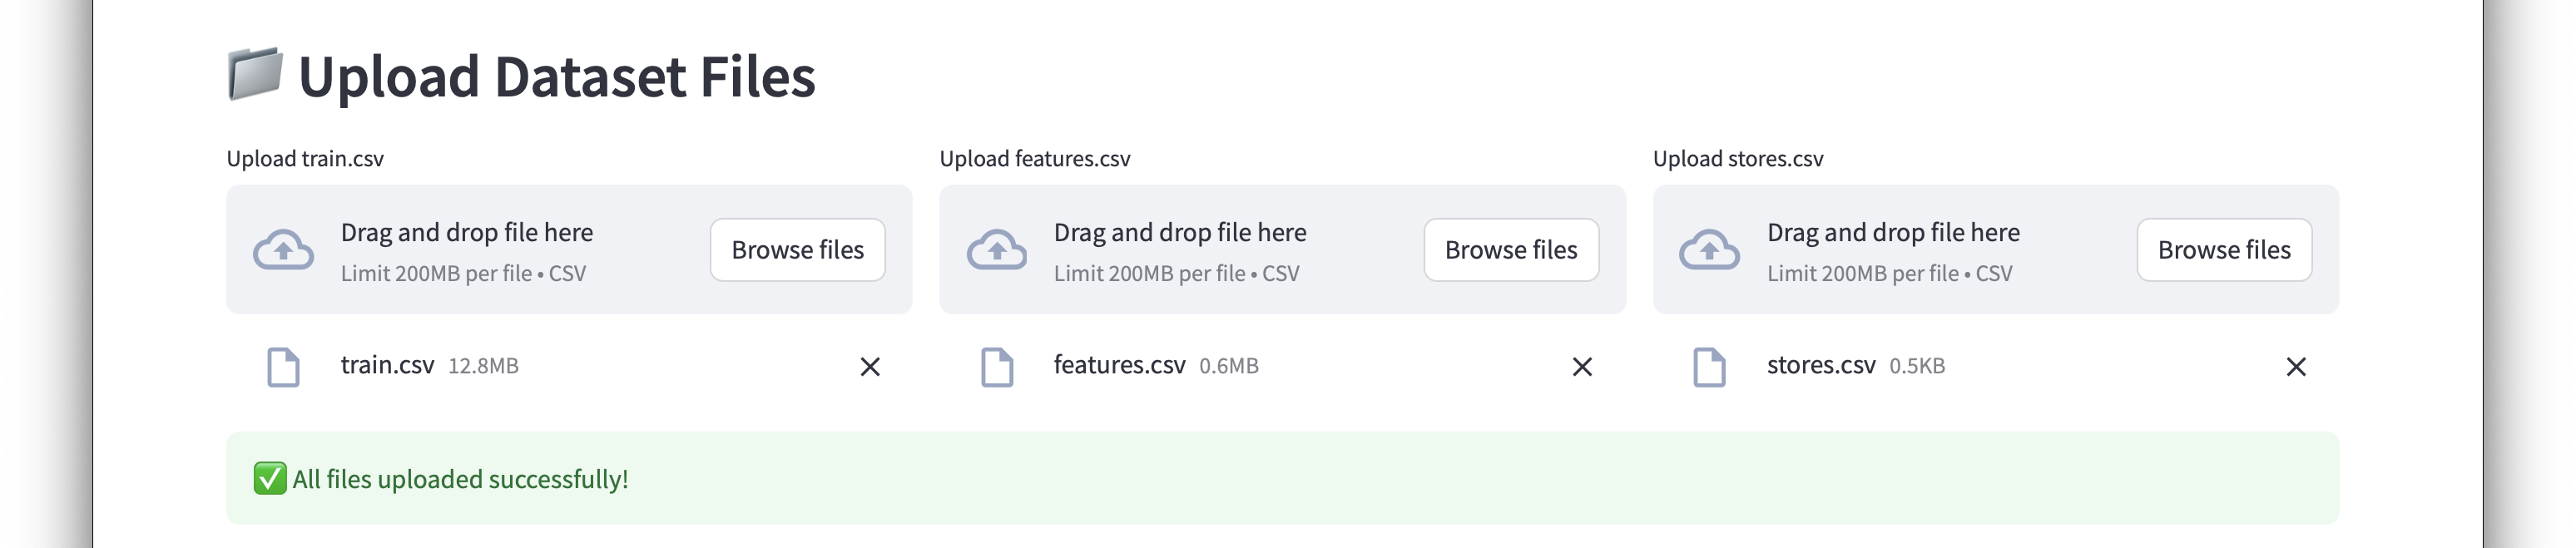
\includegraphics[width=0.9\textwidth]{Images/05ApplicationFunctionsAndFeatures/DataUpload.png}
	\caption{Multi-File Data Upload Interface}
	\label{fig:data_upload}
\end{figure}

\subsubsection{Automated Data Preprocessing}

\textbf{Data Cleaning Pipeline}
\begin{itemize}
	\item \textbf{Missing Value Imputation}: Automatic filling of missing markdown values with zeros
	\item \textbf{Outlier Detection}: Removal of negative or invalid sales records
	\item \textbf{Date Standardization}: Automatic conversion to standard date formats
	\item \textbf{Data Type Validation}: Ensures numeric columns contain valid numbers
\end{itemize}

\textbf{Feature Engineering}
\begin{itemize}
	\item \textbf{Holiday Indicators}: Automatic creation of binary holiday features
	\item \textbf{Seasonal Components}: Detection and encoding of seasonal patterns
	\item \textbf{Trend Extraction}: Identification of long-term trends in data
	\item \textbf{Merge Operations}: Intelligent joining of train, features, and stores data
\end{itemize}

\begin{figure}[H]
	\centering
	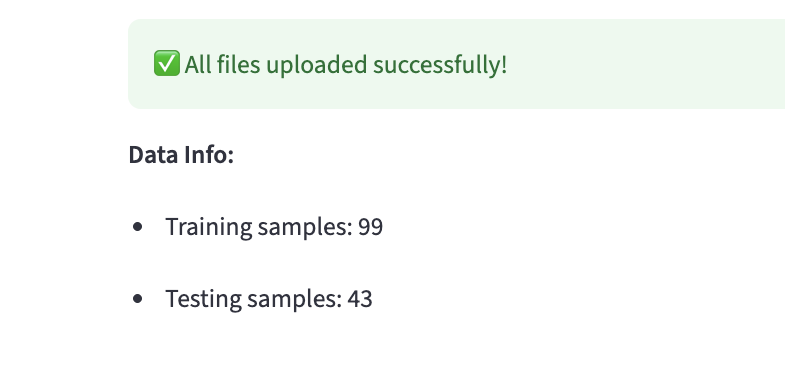
\includegraphics[width=0.9\textwidth]{Images/05ApplicationFunctionsAndFeatures/DataPreprocessing.png}
	\caption{Data Preprocessing Pipeline Results}
	\label{fig:data_preprocessing}
\end{figure}

\subsection{Model Training Functions}

\subsubsection{Auto ARIMA Training}

\textbf{Automated Parameter Selection}
\begin{itemize}
	\item \textbf{Grid Search}: Comprehensive search across parameter space
	\item \textbf{Information Criteria}: AIC-based model selection
	\item \textbf{Seasonal Detection}: Automatic identification of seasonal patterns
	\item \textbf{Differencing}: Automatic determination of differencing order
\end{itemize}

\textbf{Configurable Hyperparameters}
\begin{itemize}
	\item \textbf{AR Terms}: start\_p (0-10), max\_p (1-30)
	\item \textbf{MA Terms}: start\_q (0-10), max\_q (1-30)
	\item \textbf{Seasonal AR}: start\_P (0-10), max\_P (1-30)
	\item \textbf{Seasonal MA}: start\_Q (0-10), max\_Q (1-30)
\end{itemize}

\begin{figure}[H]
	\centering
	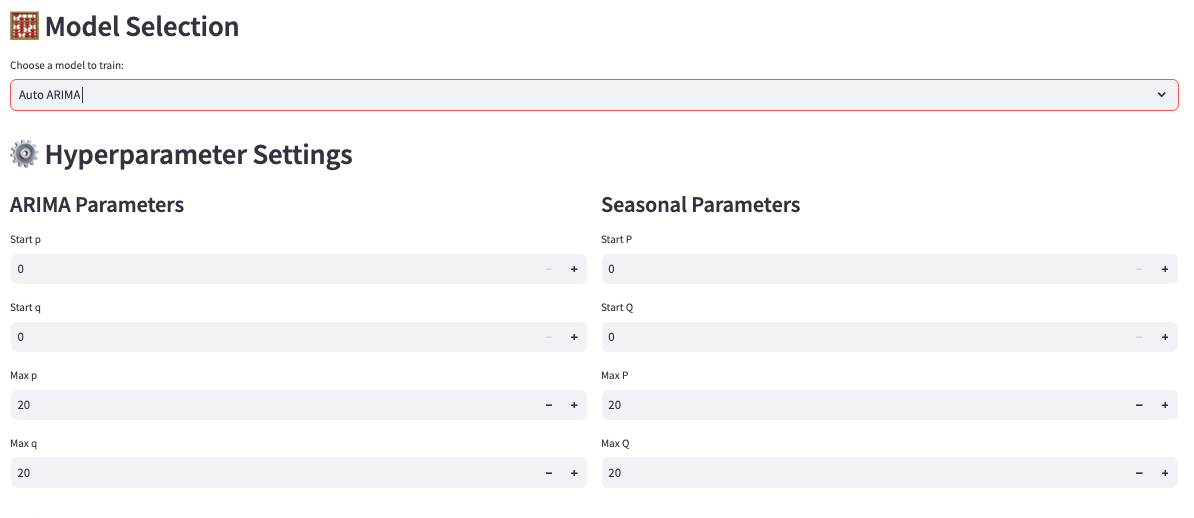
\includegraphics[width=0.9\textwidth]{Images/05ApplicationFunctionsAndFeatures/ARIMATraining.png}
	\caption{Auto ARIMA Training Configuration}
	\label{fig:arima_training}
\end{figure}

\subsubsection{Exponential Smoothing Training}

\textbf{Holt-Winters Implementation}
\begin{itemize}
	\item \textbf{Triple Smoothing}: Level, trend, and seasonal components
	\item \textbf{Additive/Multiplicative}: Choice of seasonal component type
	\item \textbf{Damped Trend}: Optional trend damping for stability
	\item \textbf{Optimization}: Automatic parameter optimization
\end{itemize}

\textbf{Seasonal Configuration}
\begin{itemize}
	\item \textbf{Seasonal Periods}: Configurable cycle length (1-52 weeks)
	\item \textbf{Seasonal Type}: Additive or multiplicative seasonality
	\item \textbf{Trend Type}: Additive, multiplicative, or none
	\item \textbf{Initialization}: Automatic initialization of smoothing parameters
\end{itemize}

\begin{figure}[H]
	\centering
	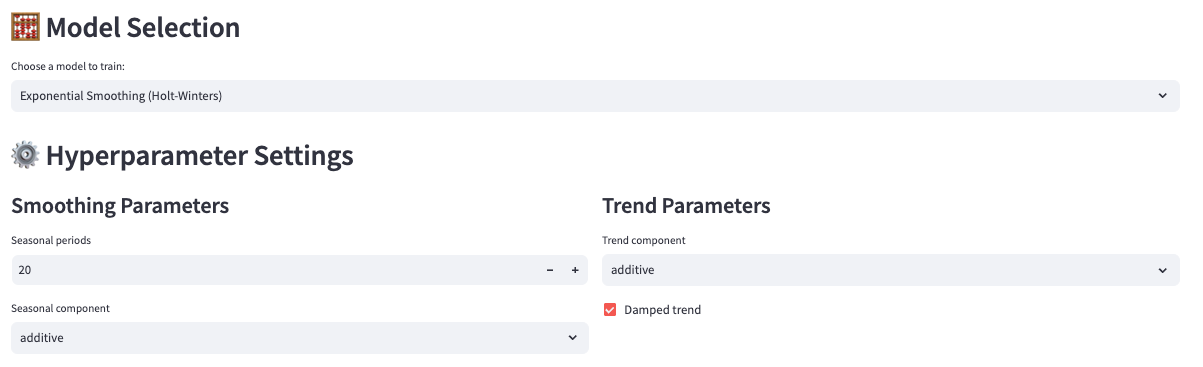
\includegraphics[width=0.9\textwidth]{Images/05ApplicationFunctionsAndFeatures/ExponentialSmoothingTraining.png}
	\caption{Exponential Smoothing Training Configuration}
	\label{fig:exponential_smoothing_training}
\end{figure}

\subsection{Model Evaluation Features}

\subsubsection{Performance Metrics}

\textbf{WMAE Calculation}
\begin{itemize}
	\item \textbf{Absolute WMAE}: Raw error metric in sales dollars
	\item \textbf{Normalized WMAE}: Percentage error relative to total sales
	\item \textbf{Interpretive Guidance}: Automatic performance category assignment
	\item \textbf{Benchmark Comparison}: Performance relative to industry standards
\end{itemize}

\textbf{Performance Categories}
\begin{itemize}
	\item \textbf{Excellent}: < 5\% normalized WMAE (Green indicator)
	\item \textbf{Acceptable}: 5-15\% normalized WMAE (Yellow indicator)
	\item \textbf{Poor}: > 15\% normalized WMAE (Red indicator)
\end{itemize}

\begin{figure}[H]
	\centering
	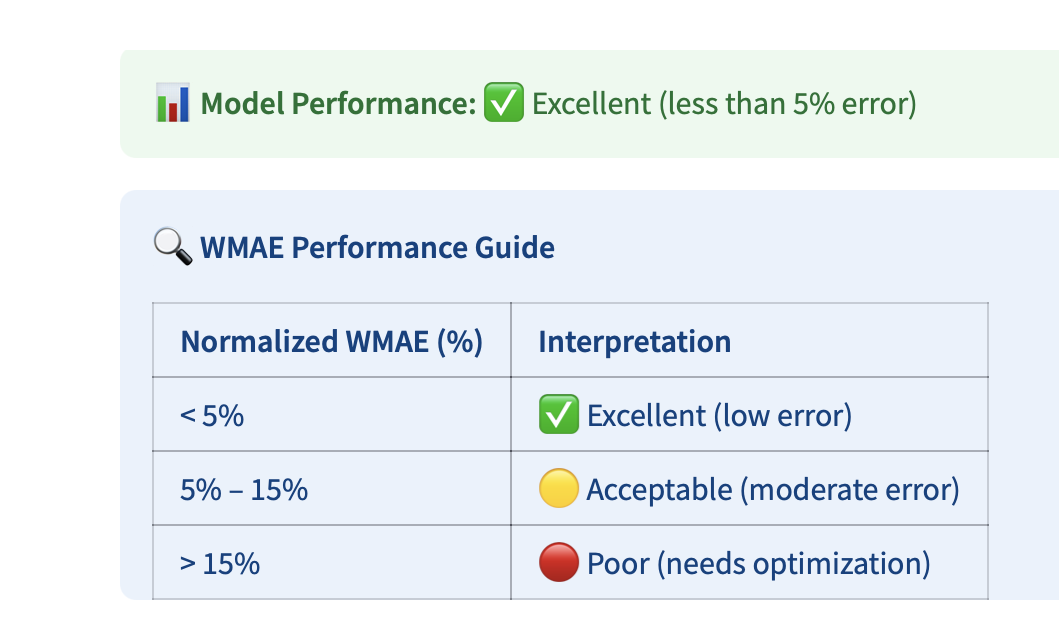
\includegraphics[width=0.9\textwidth]{Images/05ApplicationFunctionsAndFeatures/PerformanceMetrics.png}
	\caption{Model Performance Evaluation Display}
	\label{fig:performance_metrics}
\end{figure}

\subsubsection{Diagnostic Visualization}

\textbf{Training vs Testing Plots}
\begin{itemize}
	\item \textbf{Time Series Plot}: Historical data with train/test split visualization
	\item \textbf{Prediction Overlay}: Model predictions overlaid on actual test data
	\item \textbf{Residual Analysis}: Visual assessment of prediction errors
	\item \textbf{Interactive Charts}: Zoom, pan, and hover functionality
\end{itemize}

\textbf{Model Diagnostics}
\begin{itemize}
	\item \textbf{Fit Quality}: Visual assessment of model fit to training data
	\item \textbf{Prediction Accuracy}: Comparison of predictions to actual values
	\item \textbf{Trend Capture}: Evaluation of trend and seasonal pattern capture
	\item \textbf{Error Distribution}: Analysis of prediction error patterns
\end{itemize}

\begin{figure}[H]
	\centering
	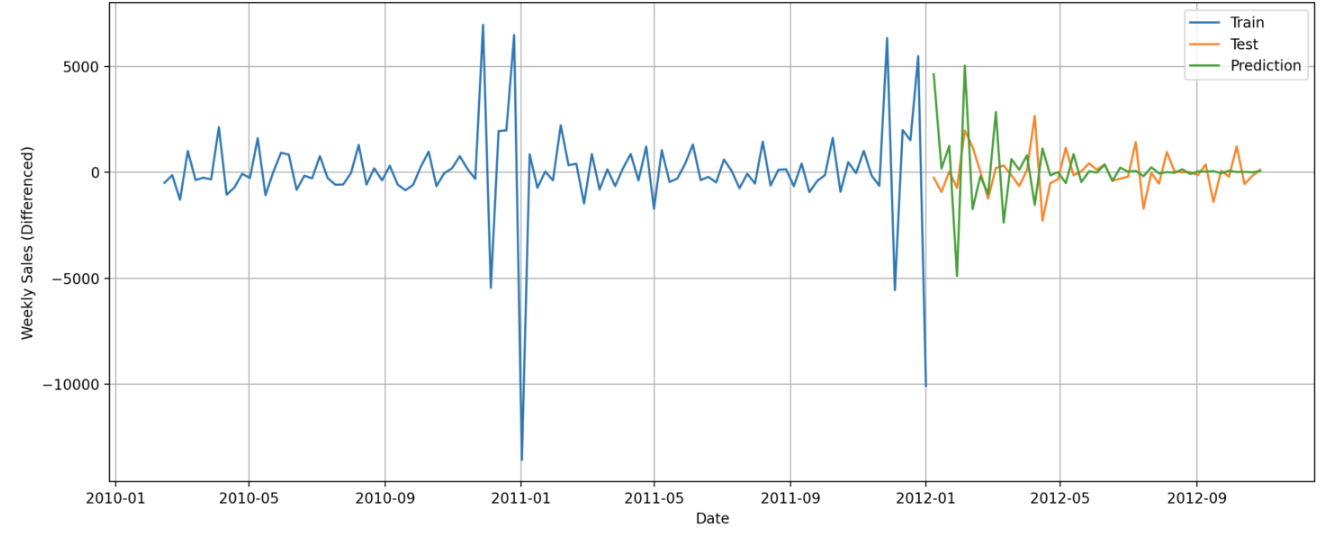
\includegraphics[width=0.9\textwidth]{Images/05ApplicationFunctionsAndFeatures/DiagnosticPlots.png}
	\caption{Comprehensive Diagnostic Visualization}
	\label{fig:diagnostic_plots}
\end{figure}

\subsection{Model Export and Management}

\subsubsection{Model Serialization}

\textbf{Export Formats}
\begin{itemize}
	\item \textbf{Primary Format}: Joblib .pkl files for cross-platform compatibility
	\item \textbf{Backup Format}: Pickle serialization as fallback option
	\item \textbf{Compression}: Efficient model compression for storage
	\item \textbf{Metadata}: Model type and performance information embedded
\end{itemize}

\textbf{File Management}
\begin{itemize}
	\item \textbf{Automatic Naming}: Descriptive filenames based on model type
	\item \textbf{Local Storage}: Models saved to models/default/ directory
	\item \textbf{Download Option}: Direct download for external use
	\item \textbf{Version Control}: Timestamp-based version management
\end{itemize}

\begin{figure}[H]
	\centering
	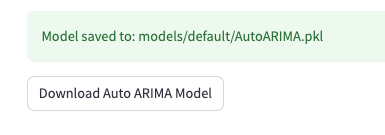
\includegraphics[width=0.9\textwidth]{Images/05ApplicationFunctionsAndFeatures/ModelExport.png}
	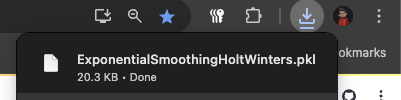
\includegraphics[width=0.9\textwidth]{Images/05ApplicationFunctionsAndFeatures/DefaultModelDownLoaded.png}
	\caption{Model Export and Download Interface}
	\label{fig:model_export}
\end{figure}

\section{Prediction Application Functions}

\subsection{Model Loading Features}

\subsubsection{Default Model Access}

\textbf{Pre-trained Model Library}
\begin{itemize}
	\item \textbf{Exponential Smoothing}: High-performance default model (3.58\% WMAE)
	\item \textbf{Performance Verification}: Pre-validated on standard datasets
	\item \textbf{Immediate Access}: One-click loading without configuration
	\item \textbf{Reliability}: Thoroughly tested and optimized parameters
\end{itemize}

\textbf{Model Specifications}
\begin{itemize}
	\item \textbf{Algorithm}: Holt-Winters Triple Exponential Smoothing
	\item \textbf{Training Data}: Comprehensive Walmart sales dataset
	\item \textbf{Seasonal Periods}: 20-week seasonal cycle optimization
	\item \textbf{Performance}: 3.58\% normalized WMAE (excellent accuracy)
\end{itemize}

\begin{figure}[H]
	\centering
	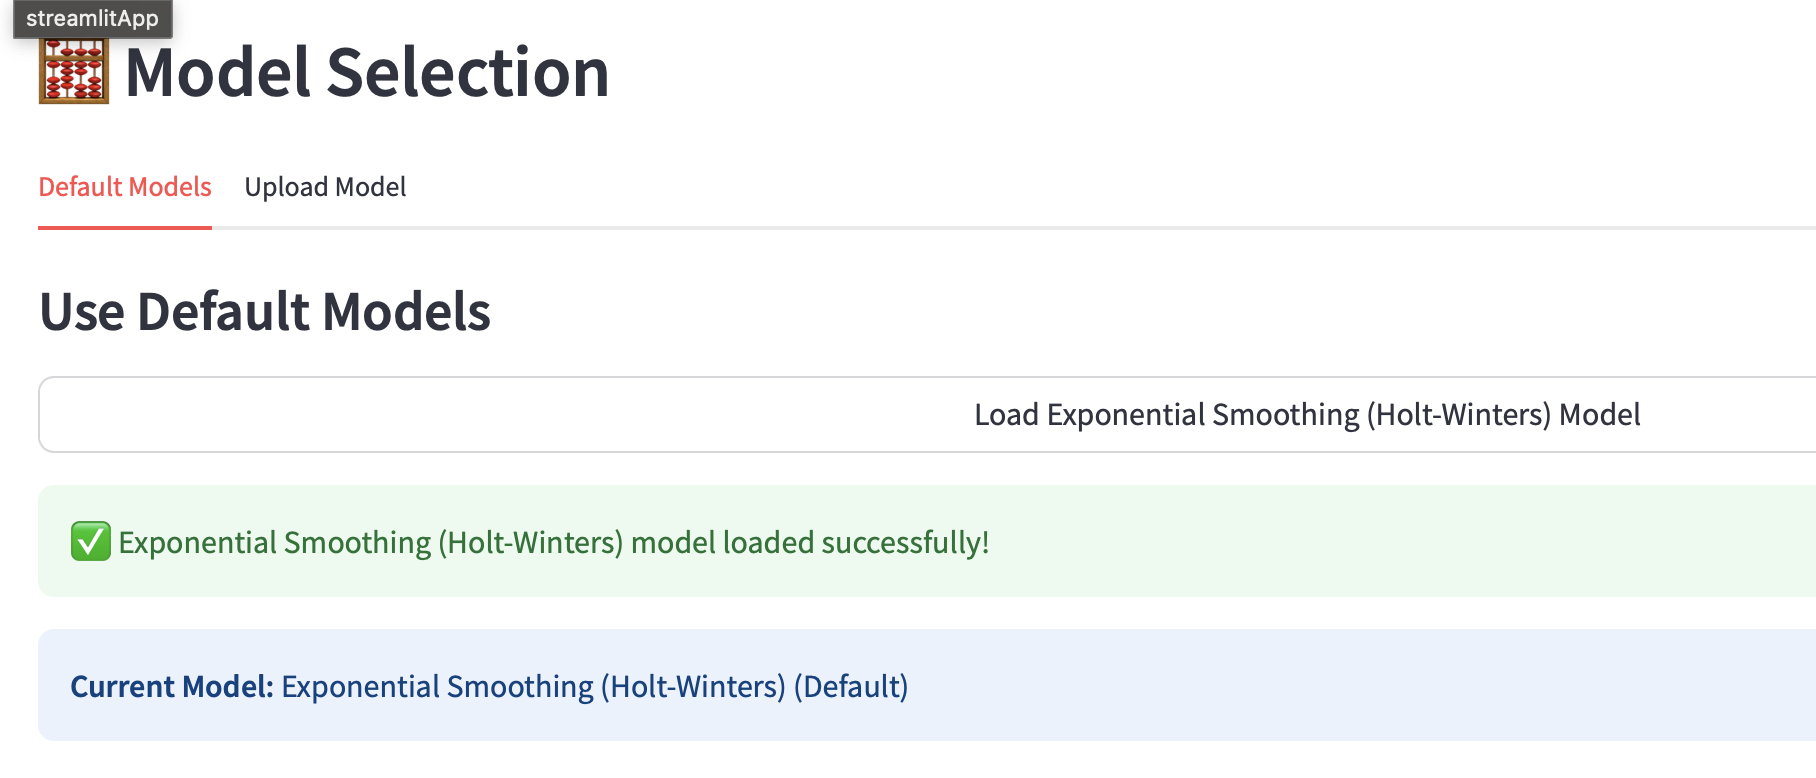
\includegraphics[width=0.9\textwidth]{Images/05ApplicationFunctionsAndFeatures/DefaultModelLoading.png}
	\caption{Default Model Loading Interface}
	\label{fig:default_model_loading}
\end{figure}

\subsubsection{Custom Model Upload}

\textbf{Model Upload Capabilities}
\begin{itemize}
	\item \textbf{File Support}: .pkl files from Training Application or external sources
	\item \textbf{Model Types}: Auto ARIMA and Exponential Smoothing support
	\item \textbf{Validation}: Automatic model format and compatibility checking
	\item \textbf{Error Handling}: Clear error messages for invalid models
\end{itemize}

\textbf{Upload Process}
\begin{enumerate}
	\item Select model type from dropdown (Auto ARIMA or Exponential Smoothing)
	\item Upload .pkl file using drag-and-drop or file browser
	\item Click "Load Uploaded Model" to validate and activate
	\item Receive confirmation message upon successful loading
\end{enumerate}

\begin{figure}[H]
	\centering
	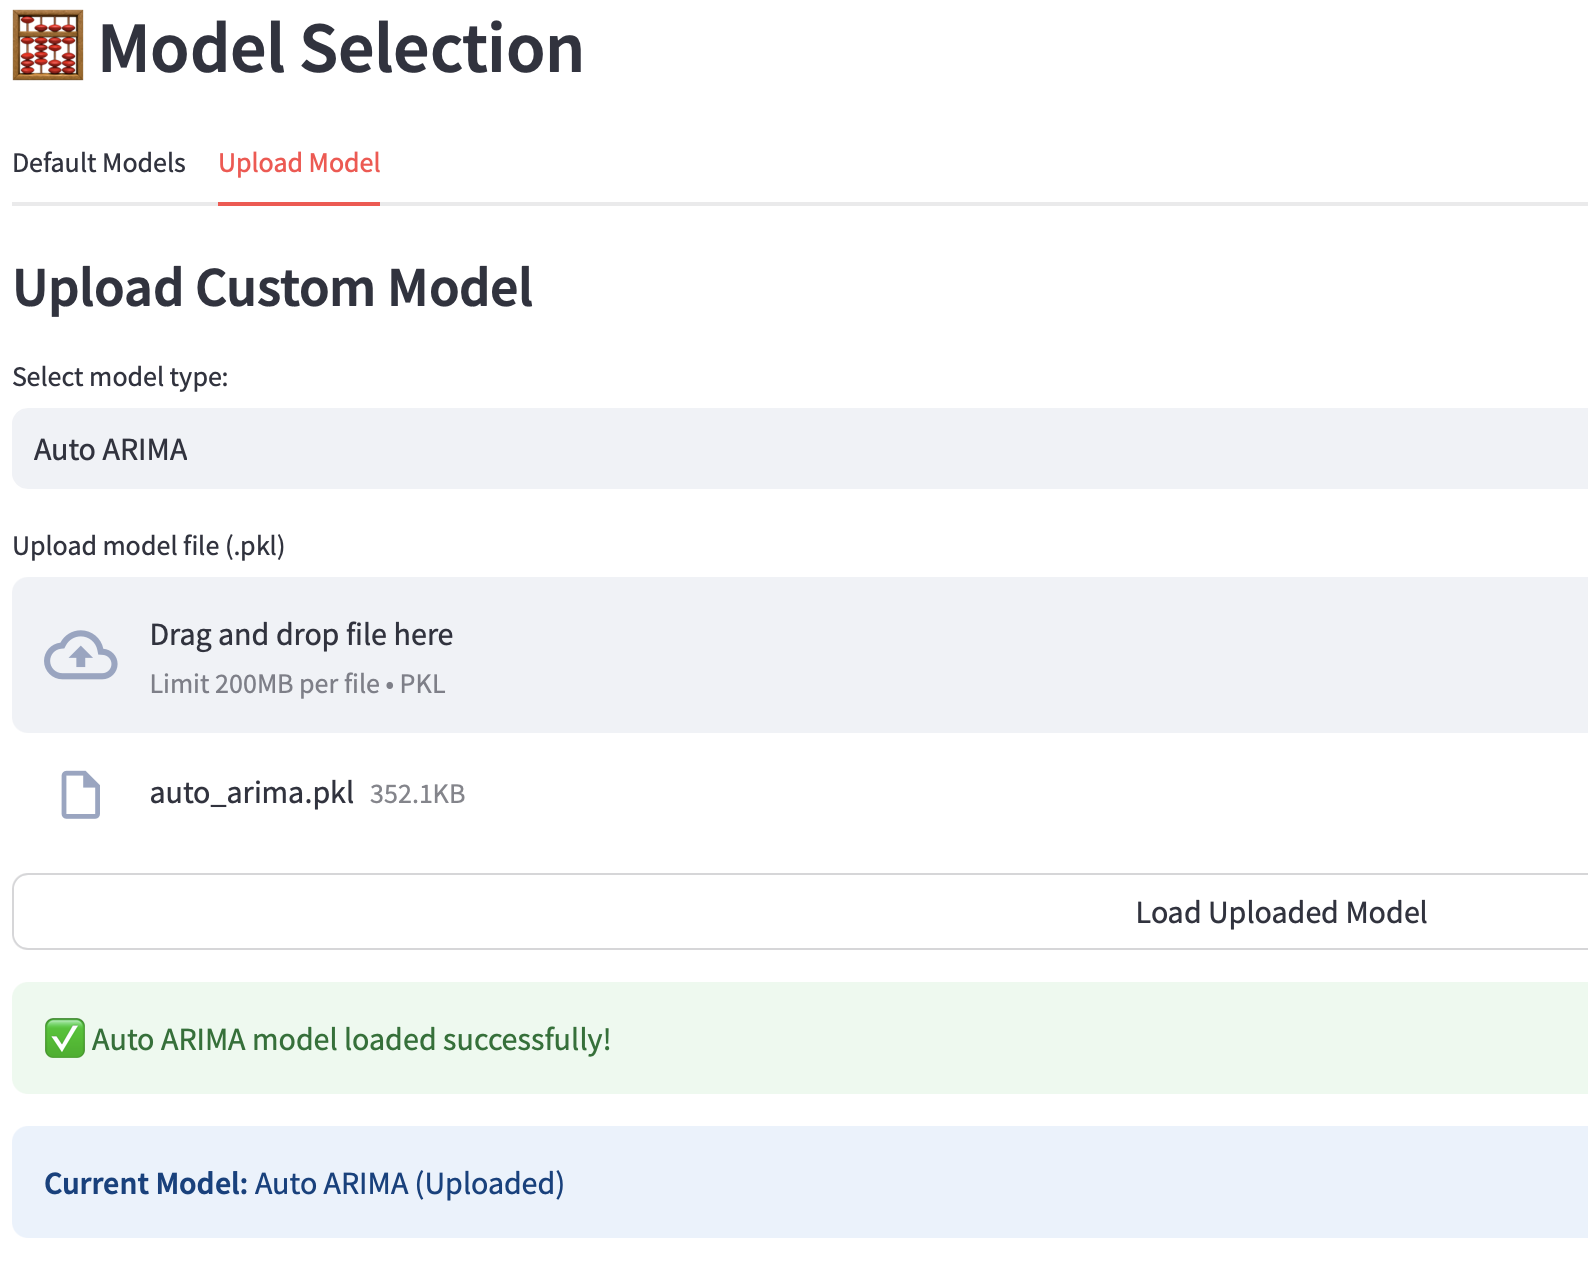
\includegraphics[width=0.9\textwidth]{Images/05ApplicationFunctionsAndFeatures/CustomModelUpload.png}
	\caption{Custom Model Upload Interface}
	\label{fig:custom_model_upload}
\end{figure}

\subsection{Forecasting Functions}

\subsubsection{Prediction Generation}

\textbf{4-Week Forecast Engine}
\begin{itemize}
	\item \textbf{Forecast Horizon}: Fixed 4-week prediction period
	\item \textbf{Output Type}: Week-over-week sales changes (not absolute values)
	\item \textbf{Processing Speed}: Sub-second prediction generation
	\item \textbf{Consistency}: Reproducible results for same model and date
\end{itemize}

\textbf{Prediction Algorithm Routing}
\begin{itemize}
	\item \textbf{Auto ARIMA}: Uses .predict() method with n\_periods parameter
	\item \textbf{Exponential Smoothing}: Uses .forecast() method with step count
	\item \textbf{Date Generation}: Automatic next-4-weeks date calculation
	\item \textbf{Error Handling}: Graceful failure with descriptive error messages
\end{itemize}

\begin{figure}[H]
	\centering
	
\includegraphics[width=0.9\textwidth]{Images/05ApplicationFunctionsAndFeatures/PredictionGeneration.png}
	\caption{Prediction Generation Process Interface}
	\label{fig:prediction_generation}
\end{figure}

\subsubsection{Results Interpretation}

\textbf{Sales Change Analysis}
\begin{itemize}
	\item \textbf{Positive Values}: Green indicators for sales increases
	\item \textbf{Negative Values}: Red indicators for sales decreases  
	\item \textbf{Magnitude Interpretation}: Dollar amounts represent change size
	\item \textbf{Baseline Reference}: Zero line for positive/negative comparison
\end{itemize}

\textbf{Business Context}
\begin{itemize}
	\item \textbf{Week-over-Week Changes}: Comparison to previous week's performance
	\item \textbf{Seasonal Patterns}: Recognition of cyclical business patterns
	\item \textbf{Trend Analysis}: Long-term direction assessment
	\item \textbf{Decision Support}: Actionable insights for business planning
\end{itemize}

\subsection{Visualization Features}

\subsubsection{Interactive Chart Display}

\textbf{Plotly-Based Visualization}
\begin{itemize}
	\item \textbf{Interactive Elements}: Hover tooltips with detailed information
	\item \textbf{Zoom Controls}: Mouse wheel and toolbar zoom functionality
	\item \textbf{Pan Navigation}: Click-and-drag chart movement
	\item \textbf{Reset View}: One-click return to default view
\end{itemize}

\textbf{Visual Design Elements}
\begin{itemize}
	\item \textbf{Color Coding}: Green bars for positive changes, red for negative
	\item \textbf{Reference Line}: Horizontal zero line for baseline comparison
	\item \textbf{Grid Lines}: Background grid for value estimation
	\item \textbf{Professional Styling}: Clean, business-appropriate chart design
\end{itemize}

\begin{figure}[H]
	\centering
	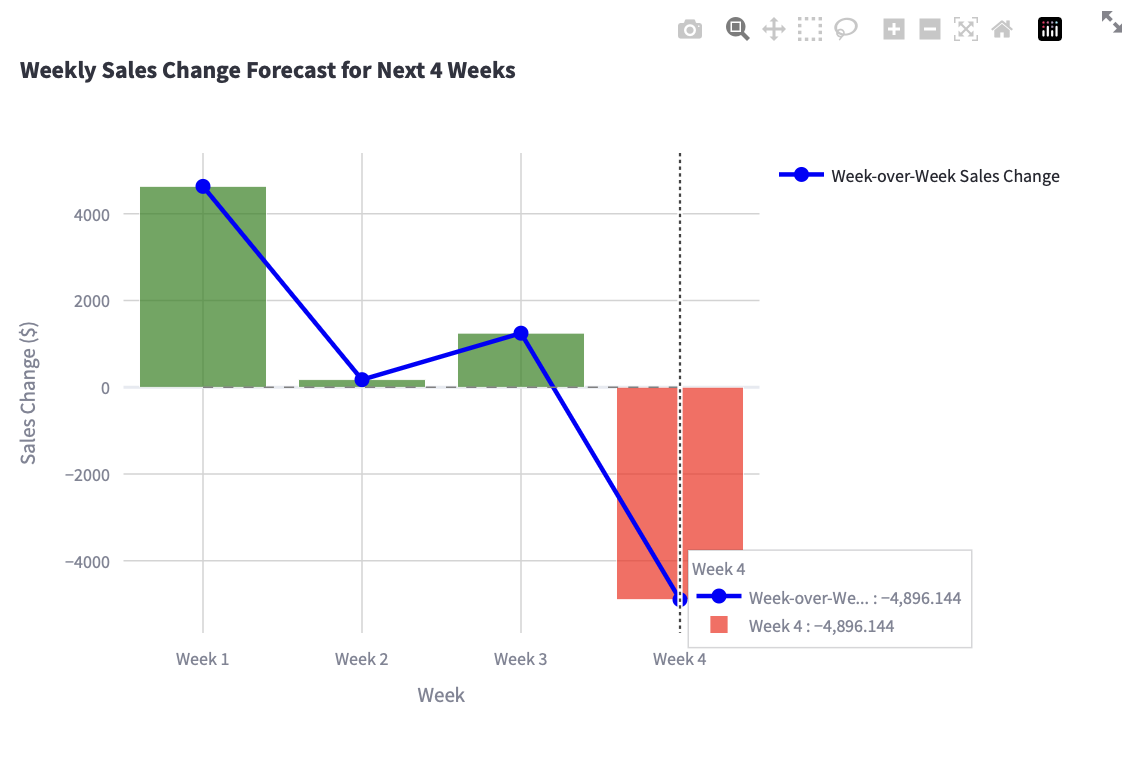
\includegraphics[width=0.9\textwidth]{Images/05ApplicationFunctionsAndFeatures/InteractiveVisualization.png}
	\caption{Interactive Chart Visualization with Controls}
	\label{fig:interactive_visualization}
\end{figure}

\subsubsection{Data Table Presentation}

\textbf{Formatted Results Display}
\begin{itemize}
	\item \textbf{Color-Coded Values}: Green text for positive, red for negative changes
	\item \textbf{Currency Formatting}: Proper dollar signs and decimal precision
	\item \textbf{Date Display}: Clear date formatting (YYYY-MM-DD)
	\item \textbf{Week Labels}: Sequential week numbering for easy reference
\end{itemize}

\textbf{Table Features}
\begin{itemize}
	\item \textbf{Responsive Design}: Adapts to different screen sizes
	\item \textbf{Clean Layout}: Minimal design focusing on data clarity
	\item \textbf{Easy Scanning}: Clear column headers and row delineation
	\item \textbf{Copy-Friendly}: Table format suitable for copying to other applications
\end{itemize}

\begin{figure}[H]
	\centering
	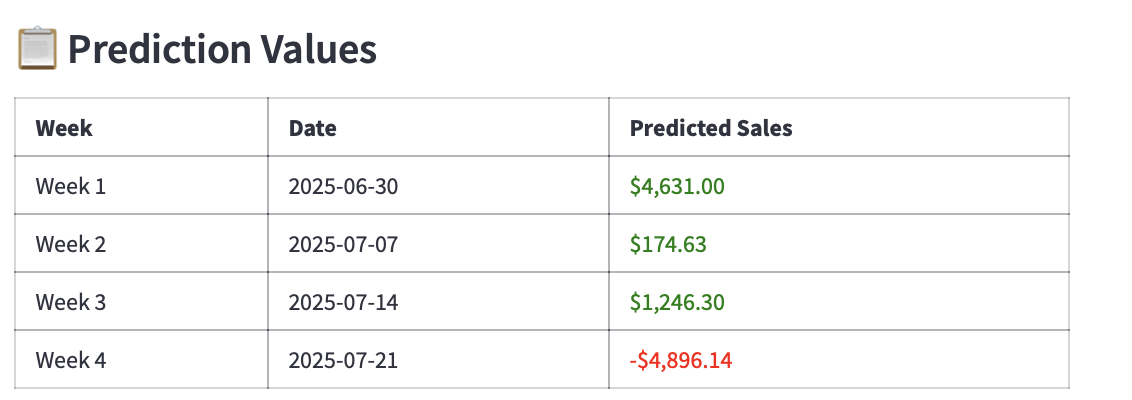
\includegraphics[width=0.9\textwidth]{Images/05ApplicationFunctionsAndFeatures/DataTablePresentation.png}
	\caption{Formatted Data Table with Color Coding}
	\label{fig:data_table_presentation}
\end{figure}

\subsection{Export and Analysis Features}

\subsubsection{Multi-Format Export}

\textbf{CSV Export}
\begin{itemize}
	\item \textbf{Standard Format}: Comma-separated values for universal compatibility
	\item \textbf{Excel Integration}: Direct opening in Microsoft Excel
	\item \textbf{Data Analysis}: Compatible with Python pandas, R, and other tools
	\item \textbf{Automatic Naming}: Descriptive filename with timestamp
\end{itemize}

\textbf{JSON Export}
\begin{itemize}
	\item \textbf{API Integration}: Machine-readable format for applications
	\item \textbf{Structured Data}: Nested format preserving data relationships
	\item \textbf{Programming Integration}: Easy import into programming environments
	\item \textbf{Web Applications}: Direct integration with web services
\end{itemize}

\begin{figure}[H]
	\centering
	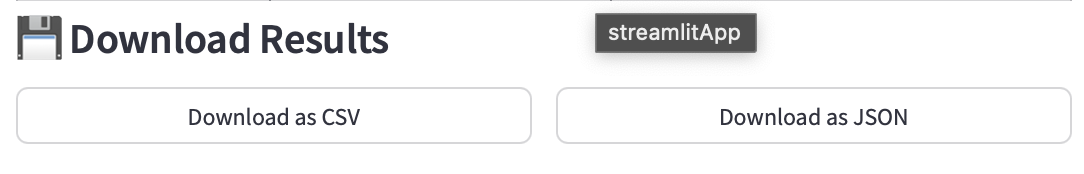
\includegraphics[width=0.9\textwidth]{Images/05ApplicationFunctionsAndFeatures/ExportFormats.png}
	\caption{Multi-Format Export Options Interface}
	\label{fig:export_formats}
\end{figure}

\subsubsection{Summary Statistics}

\textbf{Performance Metrics Display}
\begin{itemize}
	\item \textbf{Cumulative Impact}: Total sales change across all predicted weeks
	\item \textbf{Growth Week Count}: Number of weeks with positive sales changes
	\item \textbf{Best/Worst Weeks}: Identification of strongest and weakest periods
	\item \textbf{Trend Direction}: Overall forecast trend assessment
\end{itemize}

\textbf{Business Intelligence}
\begin{itemize}
	\item \textbf{Quick Insights}: At-a-glance performance summary
	\item \textbf{Decision Metrics}: Key indicators for business planning
	\item \textbf{Comparative Analysis}: Week-to-week performance comparison
	\item \textbf{Risk Assessment}: Identification of potential decline periods
\end{itemize}

\begin{figure}[H]
	\centering
	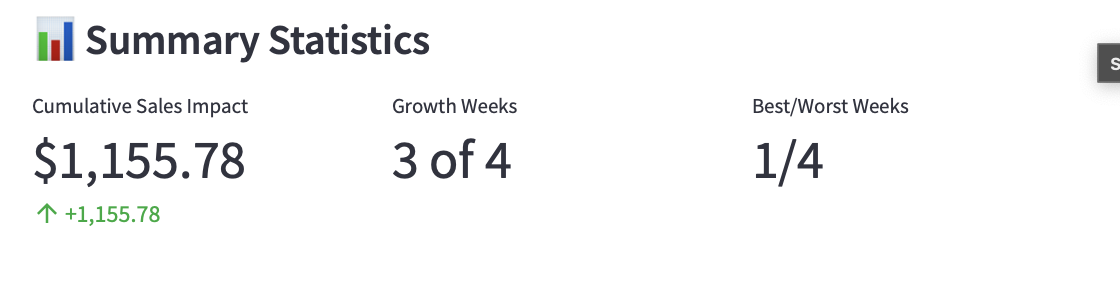
\includegraphics[width=0.9\textwidth]{Images/05ApplicationFunctionsAndFeatures/SummaryStatistics.png}
	\caption{Summary Statistics and Business Intelligence Display}
	\label{fig:summary_statistics}
\end{figure}

\section{Cross-Application Integration}

\subsection{Model Transfer Workflow}

\textbf{Training to Prediction Pipeline}
\begin{enumerate}
	\item Train model in Training Application with custom dataset
	\item Download trained model in .pkl format
	\item Upload downloaded model to Prediction Application
	\item Generate forecasts using custom-trained model
\end{enumerate}

\textbf{File Management}
\begin{itemize}
	\item \textbf{Local Installation}: Direct file copy between applications
	\item \textbf{Cloud Deployment}: Manual download/upload process
	\item \textbf{Format Consistency}: Unified .pkl format across applications
	\item \textbf{Compatibility Checking}: Automatic validation of model compatibility
\end{itemize}

\begin{figure}[H]
	\centering
	\begin{tikzpicture}[
	node distance=2.5cm,
	app/.style={rectangle, draw, fill=blue!20, text width=2.8cm, text centered, rounded corners, minimum height=1.2cm},
	process/.style={rectangle, draw, fill=green!20, text width=2.2cm, text centered, rounded corners, minimum height=0.8cm},
	file/.style={cylinder, draw, fill=yellow!20, text width=1.8cm, text centered, minimum height=0.8cm},
	arrow/.style={thick,->,>=stealth}
	]
	
	% Title
	\node[above=1.5cm] at (0,2) {\Large\textbf{Model Transfer Workflow}};
	
	% Training side
	\node[app] (training) at (-4,2) {\textbf{Training App}\\Model Development};
	\node[process] (train) at (-4,0) {Train Model\\(ARIMA/ES)};
	
	% Model file (center)
	\node[file] (model) at (0,0) {Model File\\(.pkl)};
	
	% Prediction side  
	\node[process] (forecast) at (4,-4) {Generate\\Forecast};
	\node[app] (prediction) at (4,-6) {\textbf{Prediction App}\\Forecasting};
	
	% Transfer methods
	\node[process] (local) at (-2,-2) {Local\\Copy};
	\node[process] (cloud) at (2,-2) {Download\\Upload};
	
	% Main workflow arrows
	\draw[arrow] (training) -- (train);
	\draw[arrow] (train) -- (model);
	\draw[arrow] (model) -- node[above left] {Local} (local);
	\draw[arrow] (model) -- node[above right, xshift=2cm] {      Cloud} (cloud);
	\draw[arrow] (local) -- (forecast);
	\draw[arrow] (cloud) -- (forecast);
	\draw[arrow] (forecast) -- (prediction);
	
	% Key specifications
	\node[rectangle, draw, fill=gray!10, text width=2.5cm, below=0.3cm] at (-5,-3.2) {
		\textbf{Requirements:}\\
		• .pkl format\\
		• Python 3.12\\
		• < 200MB
	};
	
	\node[rectangle, draw, fill=gray!10, text width=2.5cm, below=0.3cm] at (-1,-3.2) {
		\textbf{Performance:}\\
		• WMAPE preserved\\
		• 4-week forecast\\
		• Cross-platform
	};
	

	
\end{tikzpicture}
	\caption{Model Transfer Workflow Between Applications}
	\label{fig:model_transfer_workflow}
\end{figure}

\subsection{Workflow Optimization}

\textbf{Efficient Usage Patterns}
\begin{itemize}
	\item \textbf{Development Cycle}: Train → Evaluate → Export → Deploy → Predict
	\item \textbf{Iterative Improvement}: Compare multiple models before deployment
	\item \textbf{Performance Monitoring}: Regular retraining with new data
	\item \textbf{Version Management}: Maintain multiple model versions for comparison
\end{itemize}

\textbf{Best Practices}
\begin{itemize}
	\item \textbf{Model Documentation}: Record hyperparameters and performance metrics
	\item \textbf{Regular Updates}: Retrain models with fresh data periodically
	\item \textbf{A/B Testing}: Compare different models on same prediction tasks
	\item \textbf{Backup Strategy}: Maintain copies of well-performing models
\end{itemize}

\section{Advanced Features}

\subsection{Error Handling and Validation}

\textbf{Input Validation}
\begin{itemize}
	\item \textbf{File Format Checking}: Automatic validation of uploaded files
	\item \textbf{Data Schema Validation}: Verification of required columns and data types
	\item \textbf{Model Compatibility}: Checking model format and algorithm compatibility
	\item \textbf{Parameter Validation}: Range checking for hyperparameter inputs
\end{itemize}

\textbf{Error Recovery}
\begin{itemize}
	\item \textbf{Graceful Degradation}: Continued operation despite minor errors
	\item \textbf{Clear Error Messages}: Descriptive explanations of problems
	\item \textbf{Recovery Suggestions}: Specific steps to resolve issues
	\item \textbf{Fallback Options}: Alternative approaches when primary methods fail
\end{itemize}

\subsection{Performance Optimization}

\textbf{Computational Efficiency}
\begin{itemize}
	\item \textbf{Caching}: Intelligent caching of intermediate results
	\item \textbf{Lazy Loading}: Loading data and models only when needed
	\item \textbf{Memory Management}: Efficient memory usage for large datasets
	\item \textbf{Processing Optimization}: Streamlined algorithms for faster execution
\end{itemize}

\textbf{User Experience Enhancement}
\begin{itemize}
	\item \textbf{Progress Indicators}: Real-time feedback during long operations
	\item \textbf{Asynchronous Processing}: Non-blocking user interface during computation
	\item \textbf{Session Management}: Maintaining state across user interactions
	\item \textbf{Responsive Design}: Adaptive interface for different devices
\end{itemize}

\section{Feature Comparison Matrix}

\begin{table}[H]
	\centering
	\begin{tabularx}{\textwidth}{|X|c|c|}
		\hline
		\textbf{Feature} & \textbf{Training App} & \textbf{Prediction App} \\
		\hline
		Data Upload & Yes (Multi-file) & No \\
		Model Training & Yes (ARIMA, ES) & No \\
		Custom Models & Yes (Export) & Yes (Import) \\
		Default Models & No & Yes \\
		Hyperparameter Tuning & Yes & No \\
		Performance Evaluation & Yes (WMAE) & No \\
		Forecasting & No & Yes (4-week) \\
		Visualization & Yes (Diagnostics) & Yes (Interactive) \\
		Export Options & Yes (Models) & Yes (Results) \\
		Cloud Access & Yes & Yes \\
		Local Installation & Yes & Yes \\
		\hline
	\end{tabularx}
	\caption{Comprehensive Feature Comparison Between Applications}
	\label{tab:feature_comparison}
\end{table}

This comprehensive feature overview demonstrates the system's capabilities for complete time series forecasting workflows. The next chapter will detail the technical specifications and requirements for optimal system performance.